% ------------------------------------------------------------------------
%                                Capítulo 2
% ------------------------------------------------------------------------
\chapter{Detección de rayos cósmicos}
%\chapter{Marco teórico}
% ------------------------------------------------------------------------
%%Esta sección tiene como propósito presentar la información necesaria para contextualizar el proyecto y revisar el estado del arte.

\section{Rayos Cósmicos}
Los rayos cósmicos primarios son partículas procedentes del espacio cuya energía se debe a su gran velocidad.
Éstas son principalmente nucleos atómicos, fotones y partículas neutras.

Cuando los rayos cósmicos primarios interactúan con la atmósfera terrestre desencadenan un proceso estocástico conocido como lluvia atmosférica extendida (EAS, por sus siglas en inglés).
Esta consiste en una cascada de partículas secundarias (radiación electromagnética de muones y nucleones) que se dirigen hacia la superficie de la Tierra a altas velocidades en la dirección del rayo cósmico incidente ~\citep{ASOREY2012}.
Esta cascada es producida por la interacción de un rayo cósmico primario con átomos de la parte superior de la atmósfera.

%La lluvia atmosférica extendida es una cascada de radiación electromagnética de muones y nucleones producida por la interacción de un rayo cósmico primario con atomos de la parte superior de la atmósfera. En la Figura~\ref{lluvia} se observa como las EAS son detectadas a nivel del suelo mediante arreglos de detectores Cherenkov de agua.

Actualmente se utilizan dos tipos de métodos para la detección de rayos cósmicos: los métodos indirectos y los directos.
En los métodos directos las partículas inciden directamente con el detector, por lo cual los dispositivos de detección se encuentran situados en satélites, globos o aviones.
Los métodos indirectos detectan la cascada de partículas secundarias producida por la interacción con la atmosfera.
Para la detección de éstas se  utilizan detectores ubicados en tierra como WCD, telescopios de fluorescencia y detectores de centelleo ~\citep{schlaepfer2003cosmic}.
En la Figura~\ref{lluvia} se observa como las EAS pueden ser detectadas a nivel del suelo mediante arreglos de detectores Cherenkov de agua.

\begin{figure}[H]
\centering
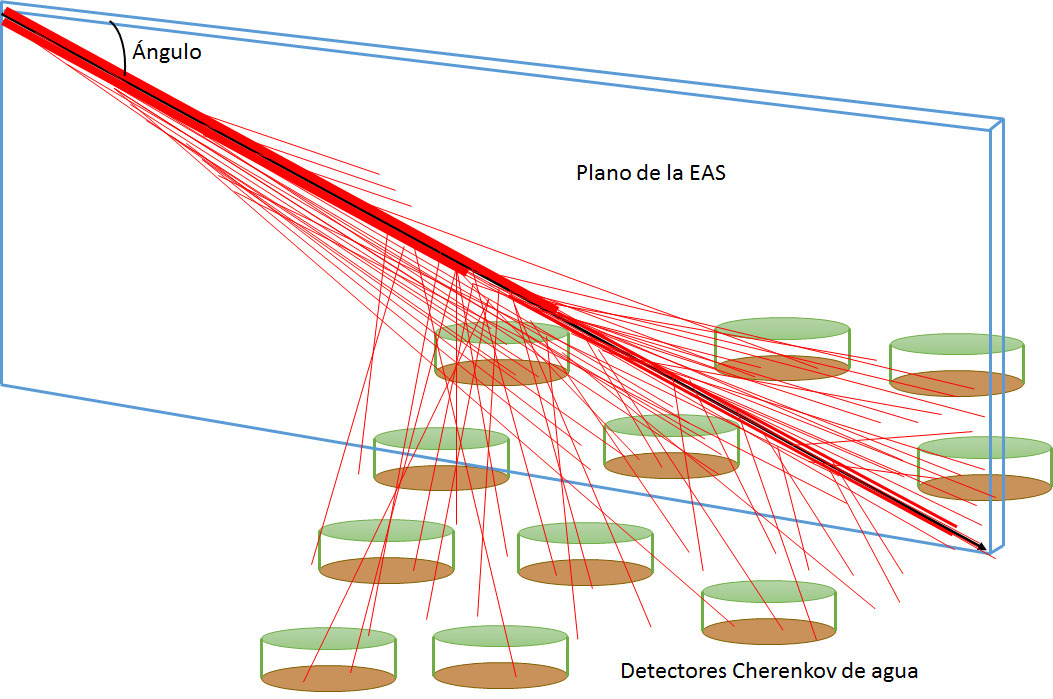
\includegraphics[width=0.8\textwidth]{Figs/imagenllu.jpeg} 
\caption[Lluvia atmósferica extendida (EAS)]
{Lluvia atmósferica extendida (EAS) detectada mediante un arreglo de varios WCD.
Procesando el tiempo con el cual el evento llega a cada detector de superficie se determina el ángulo de incidencia de las partículas.~\citep{hernandez2018procedimiento}}
\label{lluvia}
\end{figure}

\section{Proyecto LAGO}
El proyecto LAGO (por sus siglas en inglés, \textit{The Latin American Gian Observatory}) es un observatorio de astropartículas que se dedica al estudio de temas relacionados con astrofísica y clima espacial y que cuenta con equipos instalados en diferentes países de América Latina.

\subsection{Detectores WCD de LAGO}
El proyecto LAGO utiliza tanques de agua como detectores de partículas.
Un WCD típico de LAGO es un tanque lleno de agua purificada cuyo volumen oscila entre 1~$m^3$ y 40~$m^3$.
En su interior tiene una bolsa hecha por un tejido altamente difusivo y reflectante de Tyvek~\textregistered1073D para contener todo el volumen de agua y aumentar la eficiencia de detección.
El objetivo de este recubrimiento es difundir los fotones Cherenkov captados por los tubos fotomultiplicadores (PMT, por sus siglas en inglés) y reducir la dependencia de la señal de la trayectoria de las partículas secundarias dentro del detector, ya que con esto los fotones se distribuirán uniformemente dentro del tanque (Ver Figura~\ref{tank}).

\begin{figure}[H]
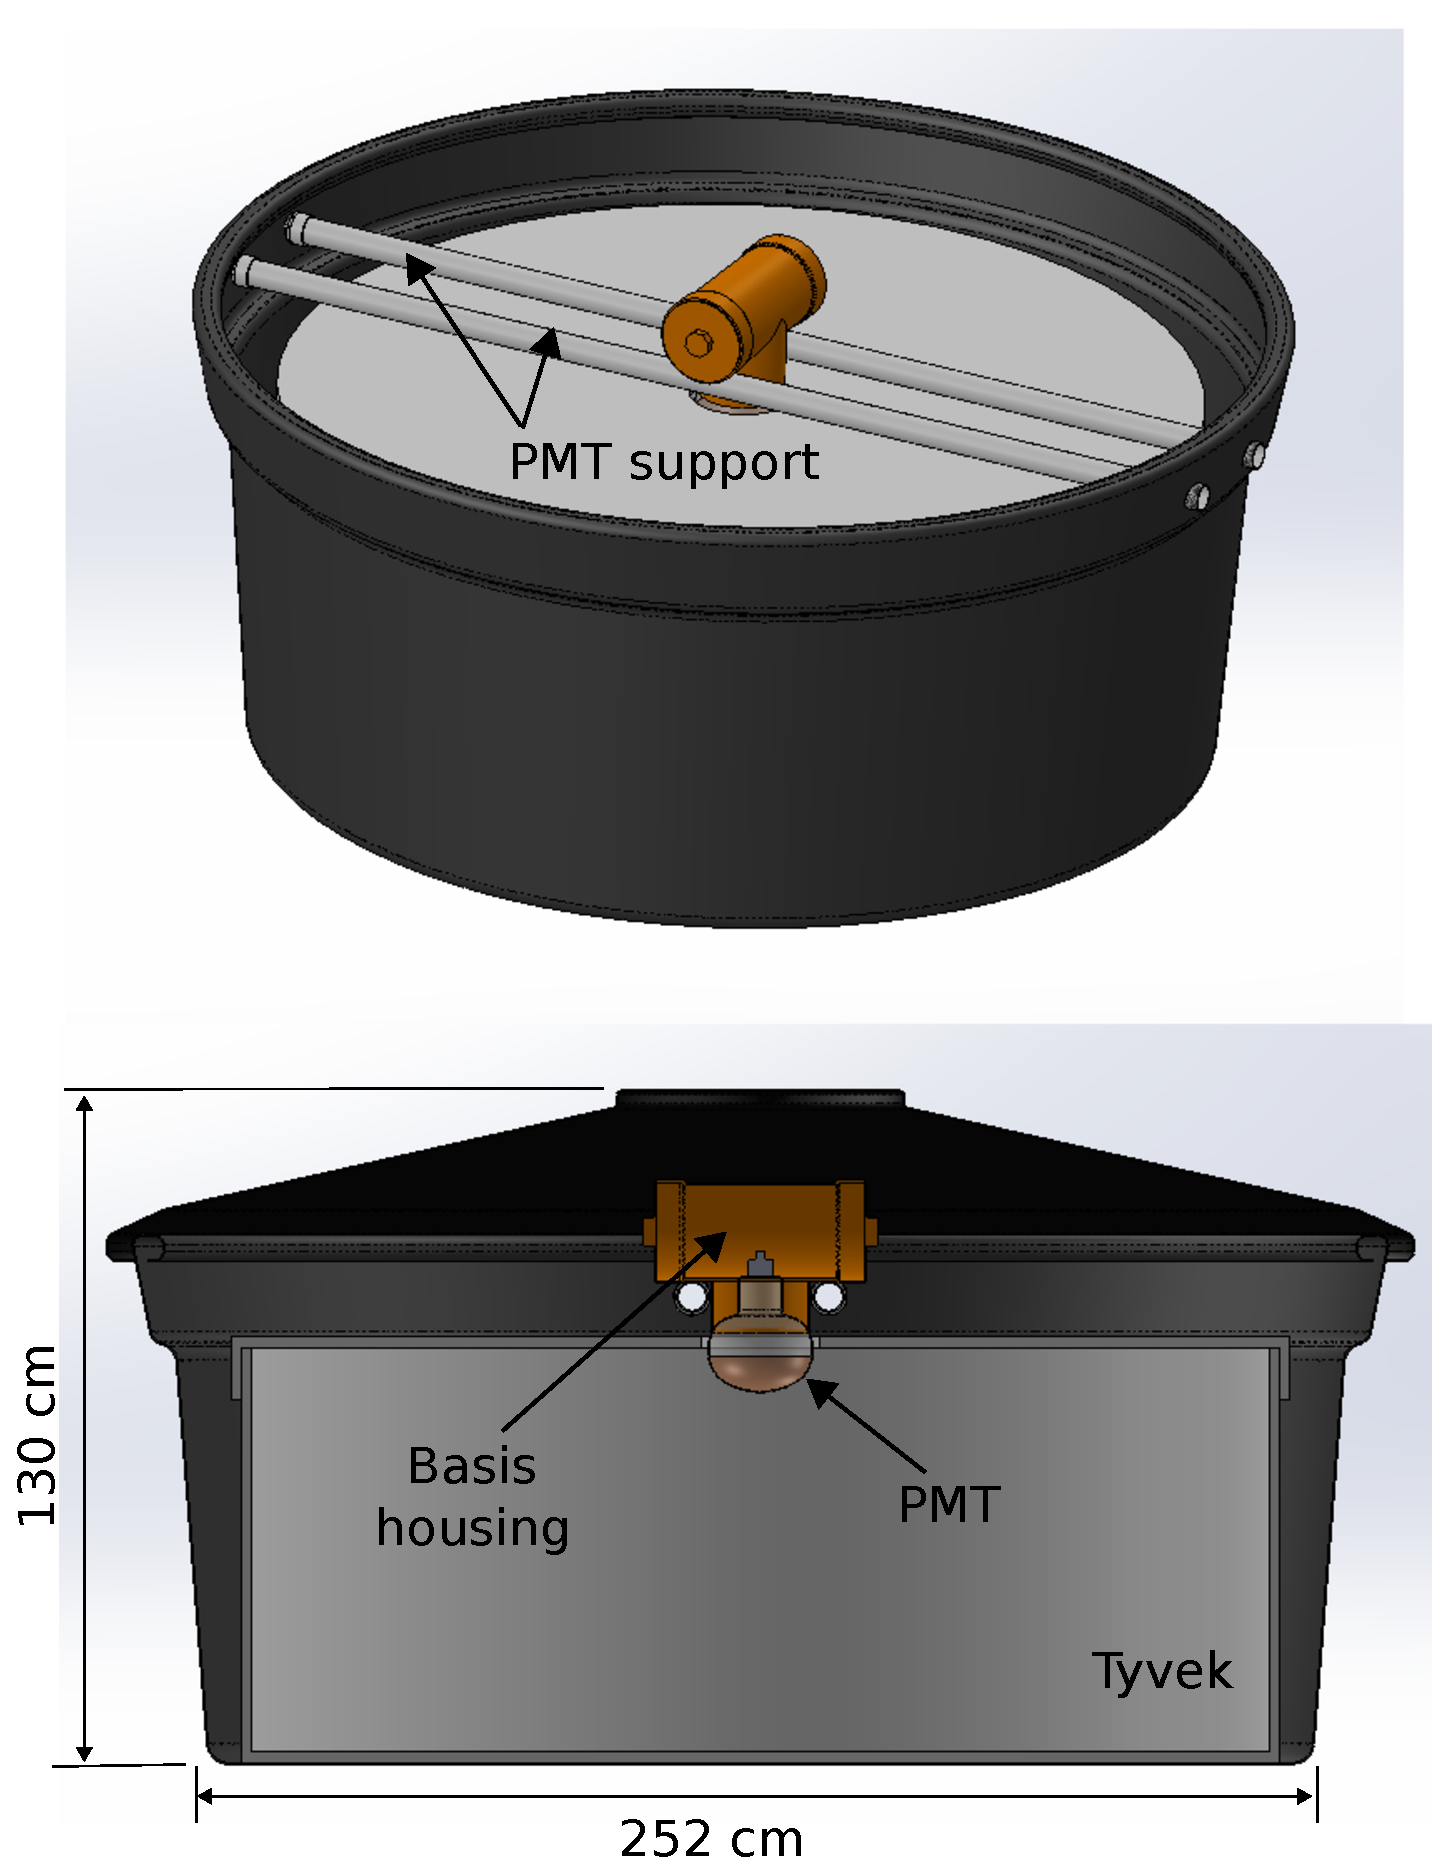
\includegraphics[scale=0.4]{Figs/Tank.eps} 
\centering
\caption{Ilustración de un Detector Cherenkov.~\citep{hernandez2018procedimiento}}
\label{tank}
\end{figure}

\subsection{Tubo fotomultiplicador}
Los PMT son los dispositivos fotosensores más empleados debido tanto a su gran versatilidad como sus características (respuesta rápida, alta sensibilidad y alto factor de ganancia).
Un tubo fotomultiplicador funciona como transductor y a su vez como amplificador, es decir, que a partir de una luz detectada se produce una corriente eléctrica fácilmente medible.

En la Figura~\ref{foto} se muestra el funcionamiento interno de un PMT.
Cuando los fotones de luz visible alcanzan el fotocátodo, éste emite fotoelectrones de baja energía.
Estos electrones son acelerados y multiplicados en campos eléctricos secuenciales aplicados entre los electrodos del PMT llamados dínodos.
En los dínodos la señal eléctrica es suficientemente grande para poder ser manejada con amplificadores y analizadores de pulsos convencionales.~\citep{kaptanoglu2018characterization}.


LAGO utiliza tubos fotomultiplicadores PMT Hamamatsu R5912 de 8 pulgadas desarrollados por Hamamatsu Photonics los cuales se encuentran ubicados sobre el volumen de agua donde inciden los fotones de Cherenkov. 
Estos PMT tienen 10 etapas enfocadas linealmente y su circuito de alimentación está constituido por un divisor de voltaje, una fuente de alimentación de alto voltaje y un preamplificador para acondicionar las amplitudes de los pulsos de salida.
La tensión de polarización del PMT está en el rango de 0~V a 2000~V respecto a tierra y puede controlarse con una baja tensión en el rango de 0~V a 5~V.

\begin{figure}[H]
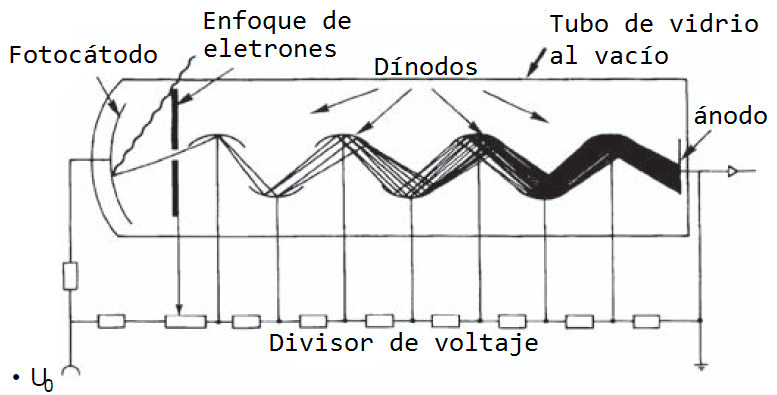
\includegraphics[scale=0.35]{Figs/pmtll.jpeg} 
\centering
\caption[Esquema de funcionamiento de un fotomultiplicador]{Esquema de funcionamiento de un fotomultiplicador.
El fotocátodo convierte la energía de luz incidente en una corriente de electrones por efecto fotoeléctrico.
El campo eléctrico creado entre los dínodos permite acelerar y guiar los electrones a lo largo del multiplicador.
El divisor de voltaje está compuesto por un arreglo de resistencias que dividen el voltaje y alimentar los dínodos.~\citep{hernandez2018procedimiento}}
\label{foto}
\end{figure}

El sistema de adquisición implementado por LAGO permite suministrar las tensiones requeridas en la base de PMT.
Un detector de WCD normalmente emite pulsos con un tiempo de subida de $\sim$10~ns y un tiempo de bajada de $\sim$70~ns.
La forma de los pulsos que vienen del detector dependen de la pureza del agua, la reflectividad del material de difusión y la geometría del tanque.~\citep{haro2016data}.
En la Figura~\ref{detec} se muestra el sistema de adquisición implementado en uno de los detectores instalado en la UIS, mientras que en la Figura~\ref{sistema_adquisicion} se muestra el diagrama de bloques de un detector WCD de LAGO.

\begin{figure}[H]
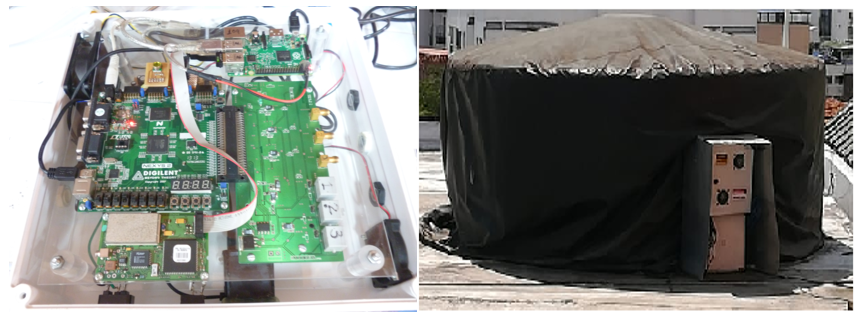
\includegraphics[scale=0.6]{Figs/lagoelectro.PNG} 
\centering
\caption[Sistema de adquisición LAGO original]{Sistema de adquisición LAGO original.
A la derecha: WCD Chitagá ubicado en Halley.
A la izquierda: electrónica del sistema de adquisición del detector.}
\label{detec}
\end{figure}

\begin{figure}[H]
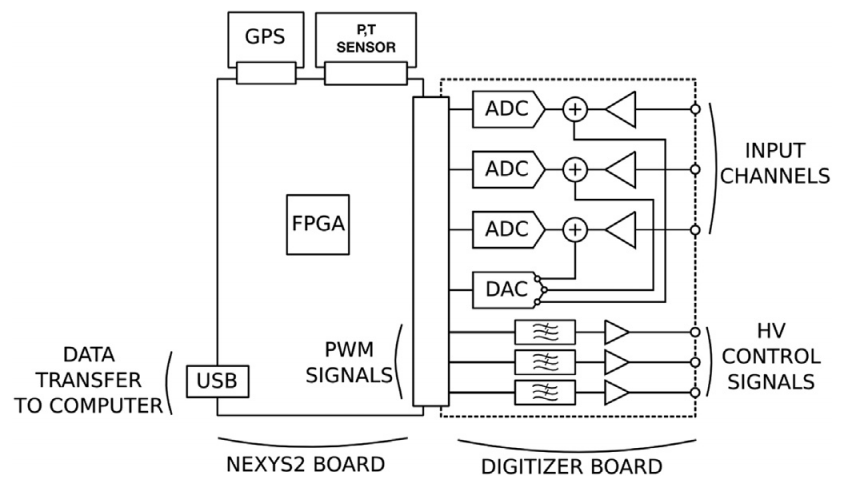
\includegraphics[scale=0.6]{Figs/bloquelago.PNG} 
\centering
\caption[Componentes principales del sistema de adquisición]{Componentes principales del sistema de adquisición: tarjeta digitalizadora de tres canales, placa Nexys-II y periféricos (GPS y sensores de temperatura y presión).~\citep{haro2016data}}.
\label{sistema_adquisicion}
\end{figure}


\begin{comment}
Existen diversos experimentos basados en la detección Cherenkov con PMTs.
A continuación se mencionan algunos de ellos.

\subsection{Kamiokande}
Ubicado en el municipio de Kamioka( Gifu, Japón) está el detector de agua Cherenkov más grande del mundo.
Este detector es operado por la Colaboración Super-Kamiokande, una colaboración conjunta de investigación entre Japón y los EEUU.
El observatorio super-kamiokande es un detector de agua cherenkov más grande del mundo.
Construido en 1991 su primera observación en 1996 ubicado en fue diseñado con el propósito de buscar la desintegración de protones y estudiar los neutrinos de diversas fuentes: el Sol, la atmósfera, las supernovas, los rayos gamma y otras fuentes astrofísicas, así como los neutrinos artificiales, así como distinguir los eventos de neutrinos de los eventos de muones de rayos cósmicos~\citep{fukuda2003super}.

El detector de agua Cherenkov Super-Kamiokande consta de un tanque de acero inoxidable, de 39~m de diámetro y 42~m de altura, con una capacidad nominal total de 50,000 toneladas de agua. 
El tanque es autoportante, con hormigón rellenado contra las paredes de piedra labrada en bruto para contrarrestar la presión del agua cuando se llena el tanque. 
Dentro del tanque, una estructura de acero inoxidable de 55  cm de grosor, espaciada aproximadamente de 2 a 2.5~m dentro de las paredes del tanque en todos los lados.
La matriz orientada hacia adentro tiene 11~146 PMT  hemisféricos Hamamatsu Tipo R3600 de 50~cm de diámetro.
Los PMT orientados hacia adentro, y el volumen de agua que ven, se denominan Detector interno (ID).
La densidad de PMTs en la ID fue tal que efectivamente el 40\% de la superficie ID cubierta por un fotocátodo.


\subsection{IceCube Neutrino Observatory}
El Observatorio de Neutrinos IceCube es un detector de neutrinos de alta energía de un kilómetro cúbico hecho de hielo Antártico del Polo Sur (Amundsen-Scott).
Fue diseñado para detectar neutrinos de las fuentes astrofísicas más violentas de nuestro universo, y a su vez ayudar a aclarar los mecanismos para la producción de rayos cósmicos de alta energía.
Los neutrinos, partículas con poca masa y carga eléctrica, pueden llegar a la Tierra sin atenuación y sin desviación por los campos magnéticos.
Los neutrinos no se observan directamente, pero cuando interactúan con el hielo producen partículas secundarias cargadas eléctricamente que a su vez emiten luz de Cherenkov la cual viaja a través del hielo más rápido que la luz en el hielo.

IceCube utiliza la  capa de hielo glacial de 2800 m de espesor como radiador Cherenkov para partículas cargadas. 
Las interacciones de neutrinos pueden crear muones de alta energía y electrones o particulas tau, que se distinguen de los muones en función del patrón de luz emitida.
La luz de Cherenkov de estas partículas es detectada por una matriz integrada de módulos ópticos digitales (DOM), cada uno de los cuales incorpora un  tubo fotomultiplicador (PMT) R7081-02 de 10 pulgadas de diámetro fabricado por Hamamatsu Photonics.
Los DOM transmiten formas de onda de señal PMT digitalizadas con marca de tiempo a las computadoras en la superficie, los sensores IceCube recogen esta luz, se digitaliza y se marca con la hora. 
Esta información se envía a las computadoras en el IceCube Lab en la superficie, que convierte los mensajes de los DOM individuales en patrones de luz que revelan la dirección y la energía de los muones y los neutrinos~\citep{abbasi2010calibration}.


\subsection{Detector Antares}
ANTARES es un detector de neutrinos basado en una cuadrícula tridimensional de tubos fotomultiplicadores (PMT) con varias líneas de detección ancladas al fondo marino a una profundidad de 2.5~km en el Mar Mediterráneo (40~km de la costa de Toulon en Francia).
El objetivo es la reconstrucción e identificación de neutrinos de alta energía de origen extraterrestre.
Los PMT registran la luz de Cherenkov inducida por leptones cargados producidos por la interacción de neutrinos con material entorno del detector.
La propagación de la luz de Cherenkov depende en gran medida de las propiedades ópticas del agua de mar, se ve alterada principalmente por la combinación de dos efectos: absorción (desaparición de fotones) y dispersión (cambio de dirección de los fotones), fusionados en el concepto de longitud de transmisión. 
La contribución de las moléculas y las partículas en suspensión en el agua a la dispersión de fotones se tiene en cuenta mediante una función de fase de dispersión.

El diseño del detector ANTARES tiene 12 líneas de detección (altura) con 25 pisos por línea. 
Cada piso comprende tripletas de módulos ópticos (OM) resistentes a alta presión. Las distancias entre pisos y líneas son de 15~m y 60~m respectivamente.
La luz de Cherenkov que emiten los leptones cargados que cruzan el detector está registrada por los OM. 
La electrónica se encuentra en un contenedor de titanio llamado módulo de control local (LCM) justo en el centro del triplete de OM.
Cada quinto está equipado con dispositivos adicionales para la multiplexación de señales, comunicación y conversión eléctrica-óptica de las señales provenientes de ese sector. 
El módulo de control de cadena (SCM) en la parte inferior de cada línea recoge el flujo de datos de la línea y lo envía a la estación costera a través del  cable electroóptico principal (MEOC) de 40~km conectado a la caja de conexiones. 
El sistema de baliza óptica (OB) consta de un conjunto de fuentes de luz (láser y LED) que se utilizan para la calibración del tiempo, pero también para realizar mediciones y monitoreo de las propiedades ópticas del agua.
Las propiedades ópticas son relevantes como parámetros de reconstrucción de pistas ya que impactan en la propagación de la luz de Cherenkov a los OM~\citep{YEPESRAMIREZ2013203}.
\end{comment}